\RequirePackage{luatex85,shellesc}
\documentclass[multi=false, varwidth=13.5cm]{standalone}
% \documentclass[multi=false]{standalone}
\usepackage{pgfplots}
\usepgfplotslibrary{units}
\usepackage{tabularx}
\usepackage[sfdefault]{FiraSans}
\usepackage[small]{eulervm}

\usetikzlibrary{patterns, intersections, calc, hobby}
\usetikzlibrary{positioning,calc,shapes}

\pgfplotsset{
    , xtick align=center
    , ytick align=center
    , unit markings=parenthesis
    , legend style={fill=none,draw=none,font=\footnotesize}
    , axis lines=left
}


\begin{document}

\edef\H{0.8}                                             
\edef\L{0.1}                                            
\edef\M{0.5}                                            

\begin{tabularx}{13.5cm}{p{4cm} p{3cm} p{5cm}}
    \textbf{A}

\begin{tikzpicture}[scale=1 , every node/.style={inner sep=1pt} ]
\begin{axis}[ xlabel=x,ylabel=E
        , enlargelimits=true
        , xtick=\empty , ytick=\empty
        , height=4cm, width=5cm 
        , ymin = 0
        , ylabel near ticks
        , xlabel near ticks
        , title = Deterministic
    ]

    %%% Use Hobby; NOTE: Don't. Looks like a human butt.
    %\addplot [color=black, smooth, very thick, hobby
    %    ] coordinates  {(0,\H) (0.1,0.5*\H) (0.25,\L) (0.5,\M) (0.75,\L) (0.9,.5*\H) (1,\H)
    %};

    \addplot+ [no marks, smooth, very thick, 
        ] coordinates  {(0,\H) (0.1,0.5*\H) (0.25,\L) (0.5,\M) (0.75,\L) (0.9,.5*\H) (1,\H)
    };

    \node[circle, ball color=red, shading=ball, anchor=south, inner sep=3pt] 
        (unstable) at (axis cs:0.5,\M) {};

    \node[above=0mm of unstable] {$\leftrightarrow$};

    \node[draw,circle %, ball color=red, shading=ball
        , dashed, anchor=south, label=below:\footnotesize stable] 
        (stableA) at (axis cs:0.25,\L) {\footnotesize A};

    \node[draw,circle %, ball color=red, shading=ball
        , dashed, anchor=south, label=below:\footnotesize stable] 
        (stableB) at (axis cs:0.75,\L) {\footnotesize B};

\end{axis}
\end{tikzpicture}
&
\textbf{B}

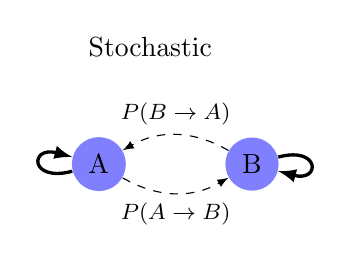
\begin{tikzpicture}[scale=1 , every node/.style={} ]
    \node[] (title) {Stochastic};

    \node[fill=blue!50, circle, below=of title.south west
        , anchor=north east 
        , xshift=5mm] (a) {A};

    \node[right=1.25cm of a, fill=blue!50, circle] (b) {B};

    \draw[-latex, dashed] (a) to[bend right] 
        node[below,sloped] {\footnotesize $P(A \rightarrow B)$} 
        (b);

    \draw[-latex, dashed] (b) to[bend right]
        node[above, sloped] {\footnotesize $P(B \rightarrow A)$} 
        (a);

    \draw[-latex, very thick] (a) to[loop left] (a);
    \draw[-latex, very thick] (b) to[loop right] (b);

\end{tikzpicture}	

& 
\textbf{C}

\begin{tikzpicture}[scale=1]
    \begin{axis}[ name=a,
            xlabel=\# Steps
            , width=5.5cm, height=3cm 
            , ytick={0.1,0.9}
            , yticklabels={A,B}
            , enlargelimits = true
            , title = A sample behaviour
        ]
        \addplot [color=blue, thick] gnuplot [ raw gnuplot ] {
            set datafile separator ',';
            plot "./bistable/data.csv" using "steps":"state";
        };
    \end{axis}
    %%\begin{axis}[rotate=-90 
    %%        , name=b,
    %%        , at={(a.south east)}
    %%        , width=3cm, height=2cm
    %%        , xtick=\empty
    %%    ]
    %%    \addplot [color=blue, thick, hist={bins=100,density}] 
    %%        table[col sep=comma]{./bistable/data.csv};
    %%\end{axis}
\end{tikzpicture}

\end{tabularx}

\end{document}

